\documentclass{beamer}

\usepackage{fontspec} 
% \usepackage{lsp-makros}
\useoutertheme{lsp}

\usepackage{lsptitle}

\def\two@digits#1{\ifnum#1<10 0\fi\number#1}
\def\mytoday{\two@digits{\number\day}.\two@digits{\number\month}.\number\year}


\usepackage{xspace,multicol}
\newcommand{\latex}{\LaTeX\xspace}
\usepackage{tikz}


\newcounter{lastpagemainpart}
\footnotesep0pt
\renewcommand{\footnoterule}{}
\usefootnotetemplate{
  \noindent
  \insertfootnotemark\insertfootnotetext}

\let\beamerfn=\footnote
\renewcommand{\footnote}[1]{%
\let\oldfnsize=\footnotesize%
\let\footnotesize=\tiny%
\beamerfn<\thebeamerpauses->{#1}%
\let\footnotesize=\oldfnsize}


\date{Eroding Dichotomies: Description, Analysis and Publishing in African Linguistics\\\today}

\usepackage{eurosym}  
 
\renewcommand{\centerline}[1]{\hfill#1\hfill\hfill\mbox{}}


\title{Open access books}
% \institute{FU Berlin}
\author[LangSci]{Sebastian Nordhoff}



\begin{document}
\lspbeamertitle

\section{Introduction}
\frame{
\frametitle{Introduction:\strut\\ Sebastian Nordhoff}
%   \includegraphics[height=.2\textheight]{./path/to/graphicsfile}
  \begin{itemize}
    \item  lives in Western Europe
    \item  worked on languages of South America (Guarani) and Asia (Sri Lanka Malay)
    \item 4 books, 30+ scholarly articles
    \item since 2014 managing director of Language Science Press
  \end{itemize}
}

\frame{
\frametitle{Introduction:\strut\\ Language Science Press}
%   \includegraphics[height=.2\textheight]{./path/to/graphicsfile}
  \begin{itemize}
    \item  Open Access publisher
    \item no fees for readers
    \item no fees for authors
    \item 30 series ranging from laboratory phonology to translation studies
    \item 185 books up to date
  \end{itemize}
}

\frame{
\frametitle{Introduction:\strut\\ Language Science Press}
  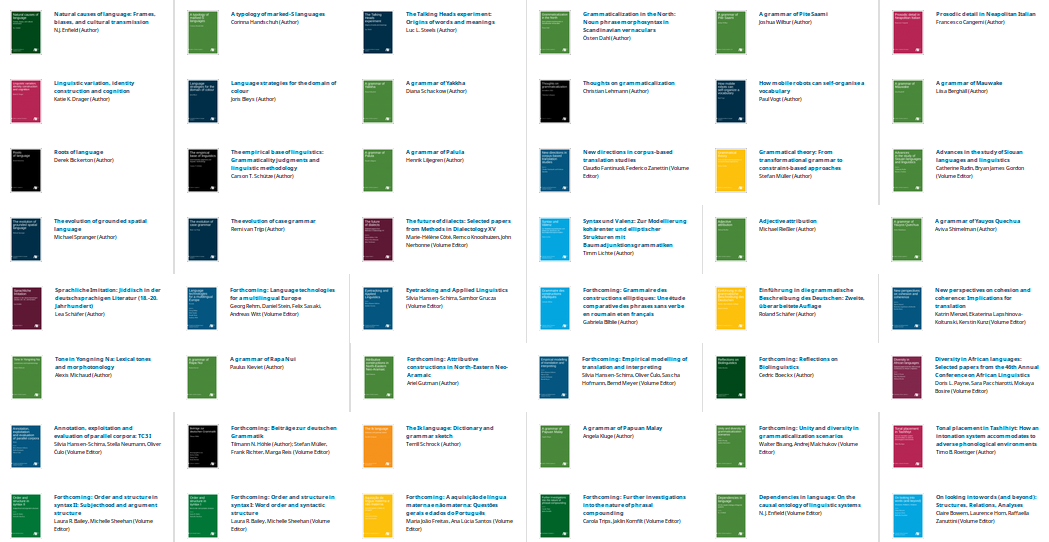
\includegraphics[height=\textheight]{catalog.png}
}

\frame{
\frametitle{Roads to Open Access}
%   \includegraphics[height=.2\textheight]{./path/to/graphicsfile}
  \begin{itemize}
    \item  \textbf{The Green Road}: repositories
    \item \textbf{The Golden Road}: author pays
    \item \textbf{The Diamond Road}: community pays
  \end{itemize}
}

\section{Articles}
\frame{
\frametitle{The Green Road}
%   \includegraphics[height=.2\textheight]{./path/to/graphicsfile}
  \begin{itemize}
    \item Choose a traditional journal
    \item Get your article accepted
    \item The journal publishes and monetizes your article as usual
    \item You deposit a version of the article in a depository of your university or a repository of your discipline
    \begin{itemize}
      \item publisher regulation vary as to which version (submitted, accepted, published) you can deposit
      \item check Sherpa Romeo https://v2.sherpa.ac.uk/romeo/search.html
    \end{itemize}
  \end{itemize}
}

\frame{
\frametitle{Sherpa Romeo}
  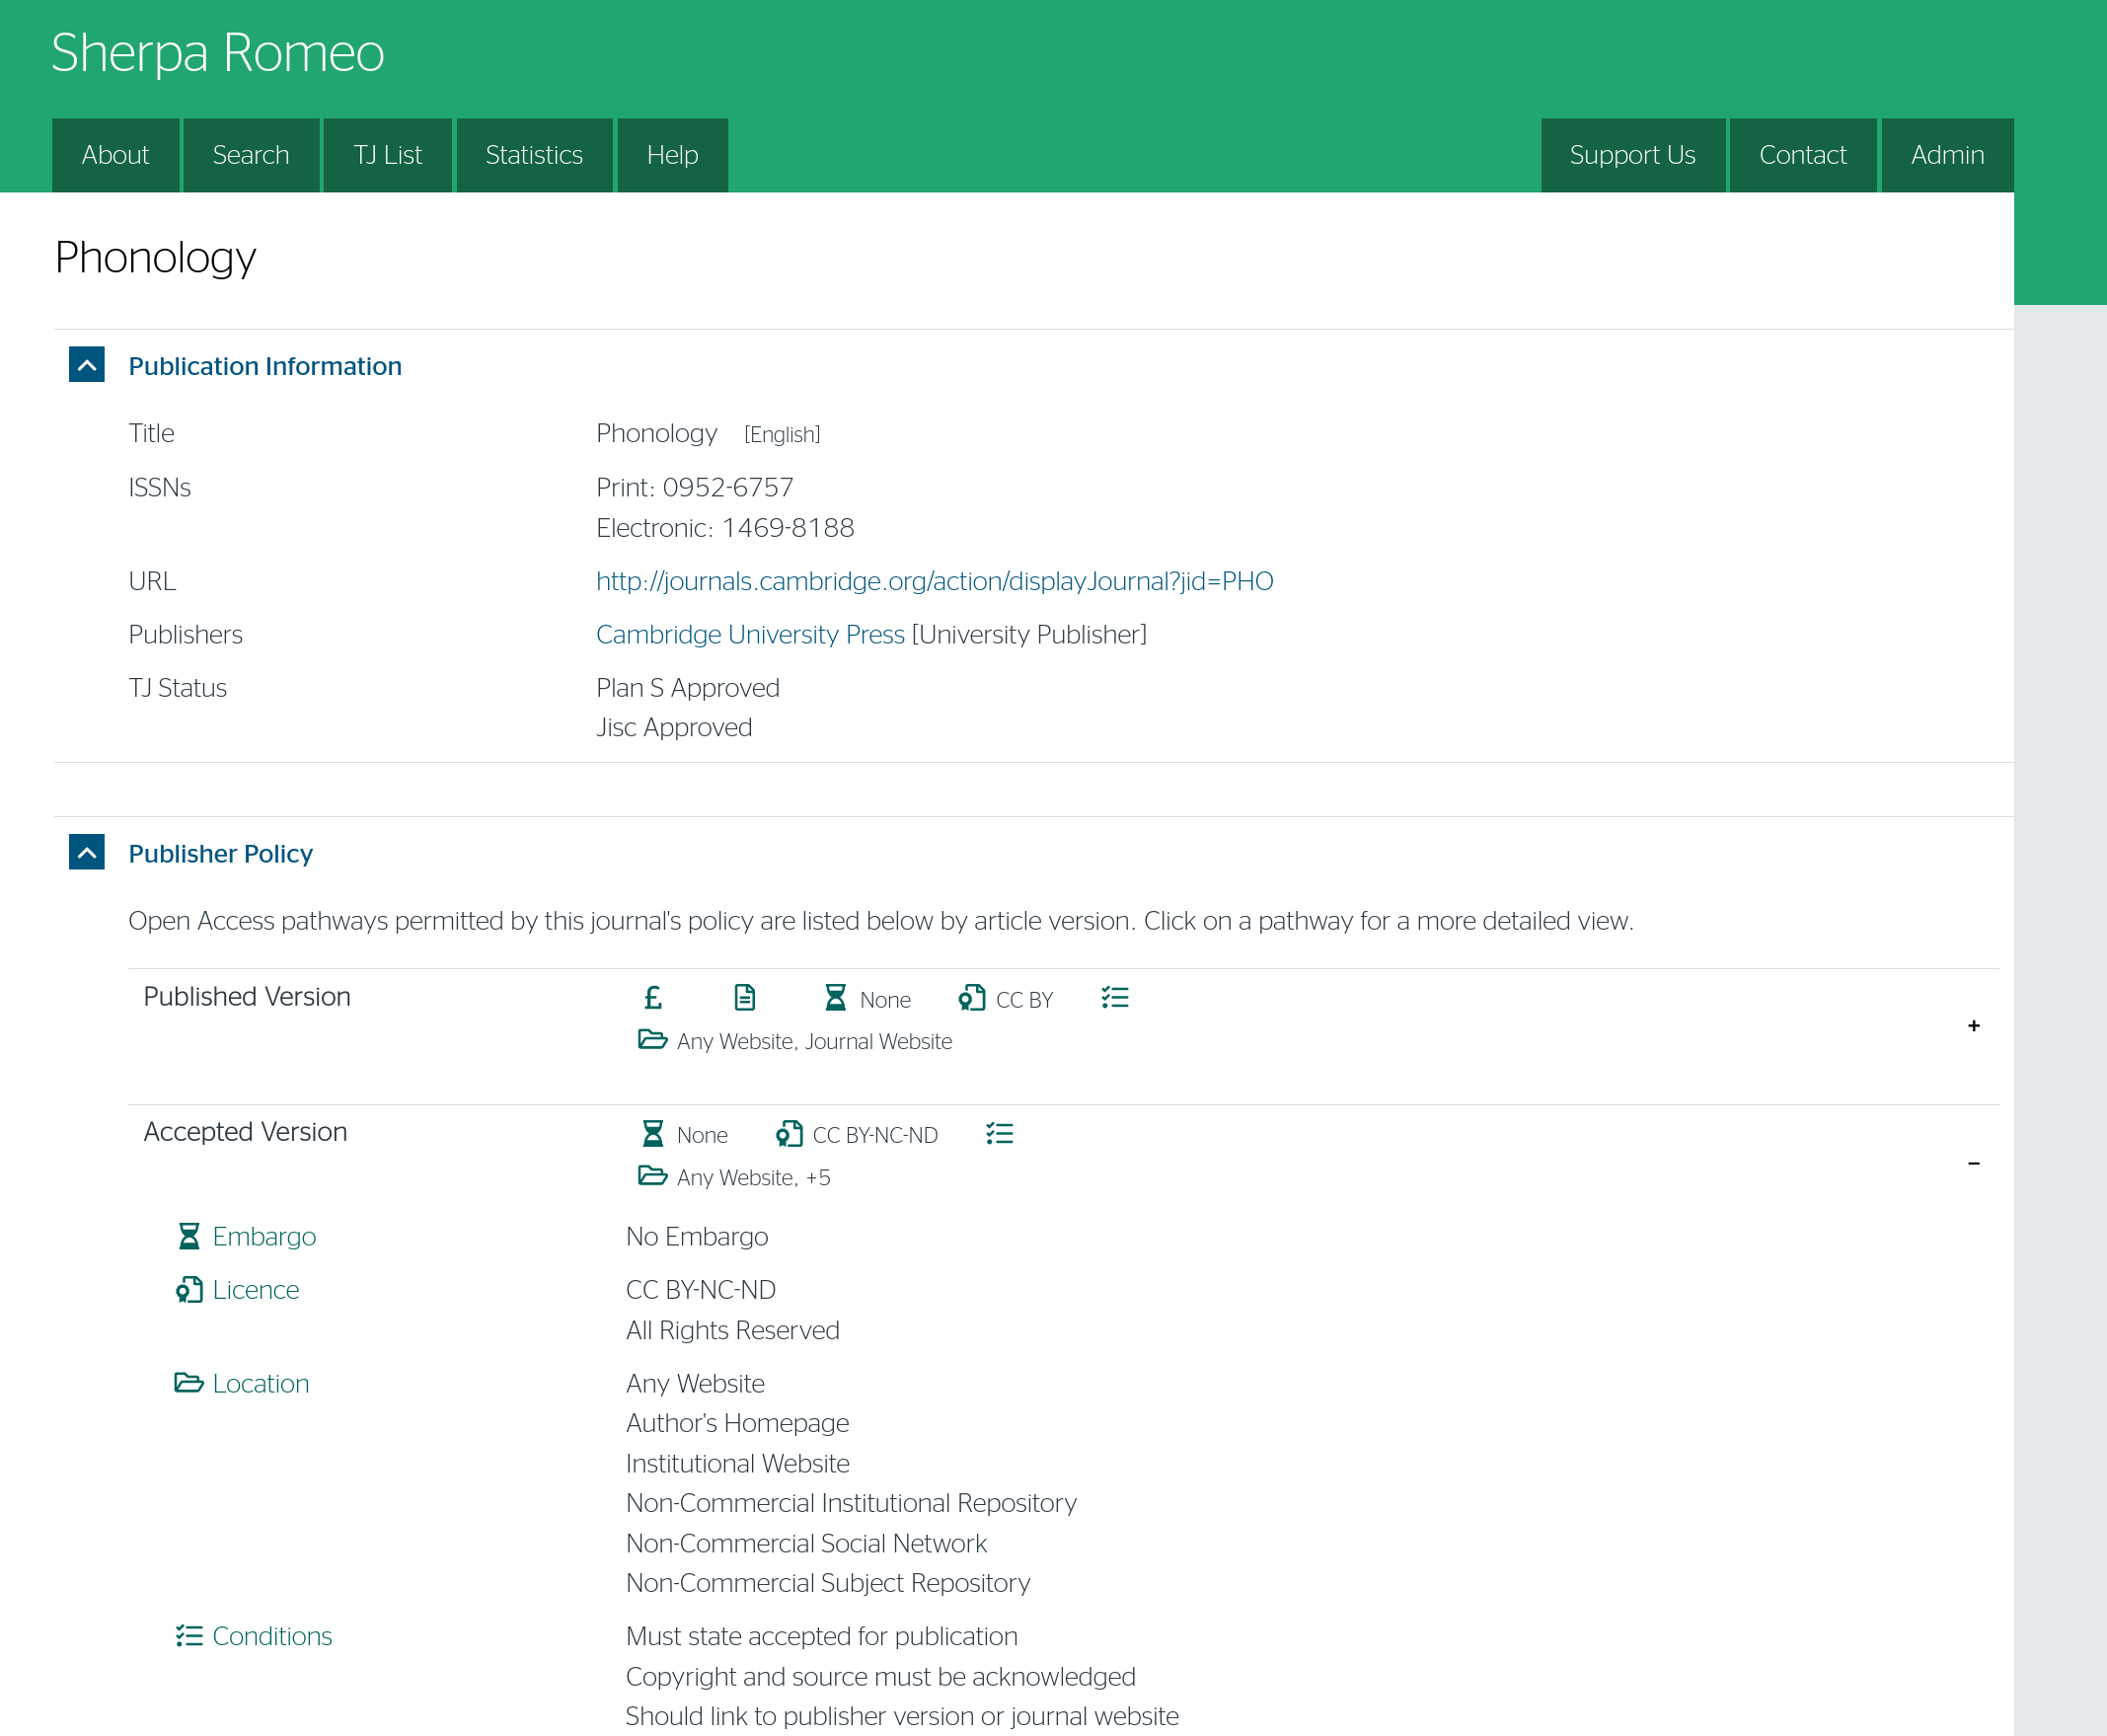
\includegraphics[height=1\textheight]{sherparomeo.png}
}

\frame{
\frametitle{The Golden Road}
%   \includegraphics[height=.2\textheight]{./path/to/graphicsfile}
  \begin{itemize}
    \item Select a journal
    \item Get your paper accepted
    \item Pay a fee
    \begin{itemize}
      \item article: 300 USD -- 3.000 USD
      \item book: 5.000 -- 25.000 USD
    \end{itemize}
    \item Readers don't have to pay anything to read the article
    \item Beware of predatory journals!
    \item Check the Directory of Open Access Journals (DOAJ)
    \item thinkchecksubmit.org
  \end{itemize}
}

\frame{
\frametitle{Predatory Journals}
  
\includegraphics[height=.45\textheight]{predatoryjournal.png}
}


\frame{
\frametitle{DOAJ}
  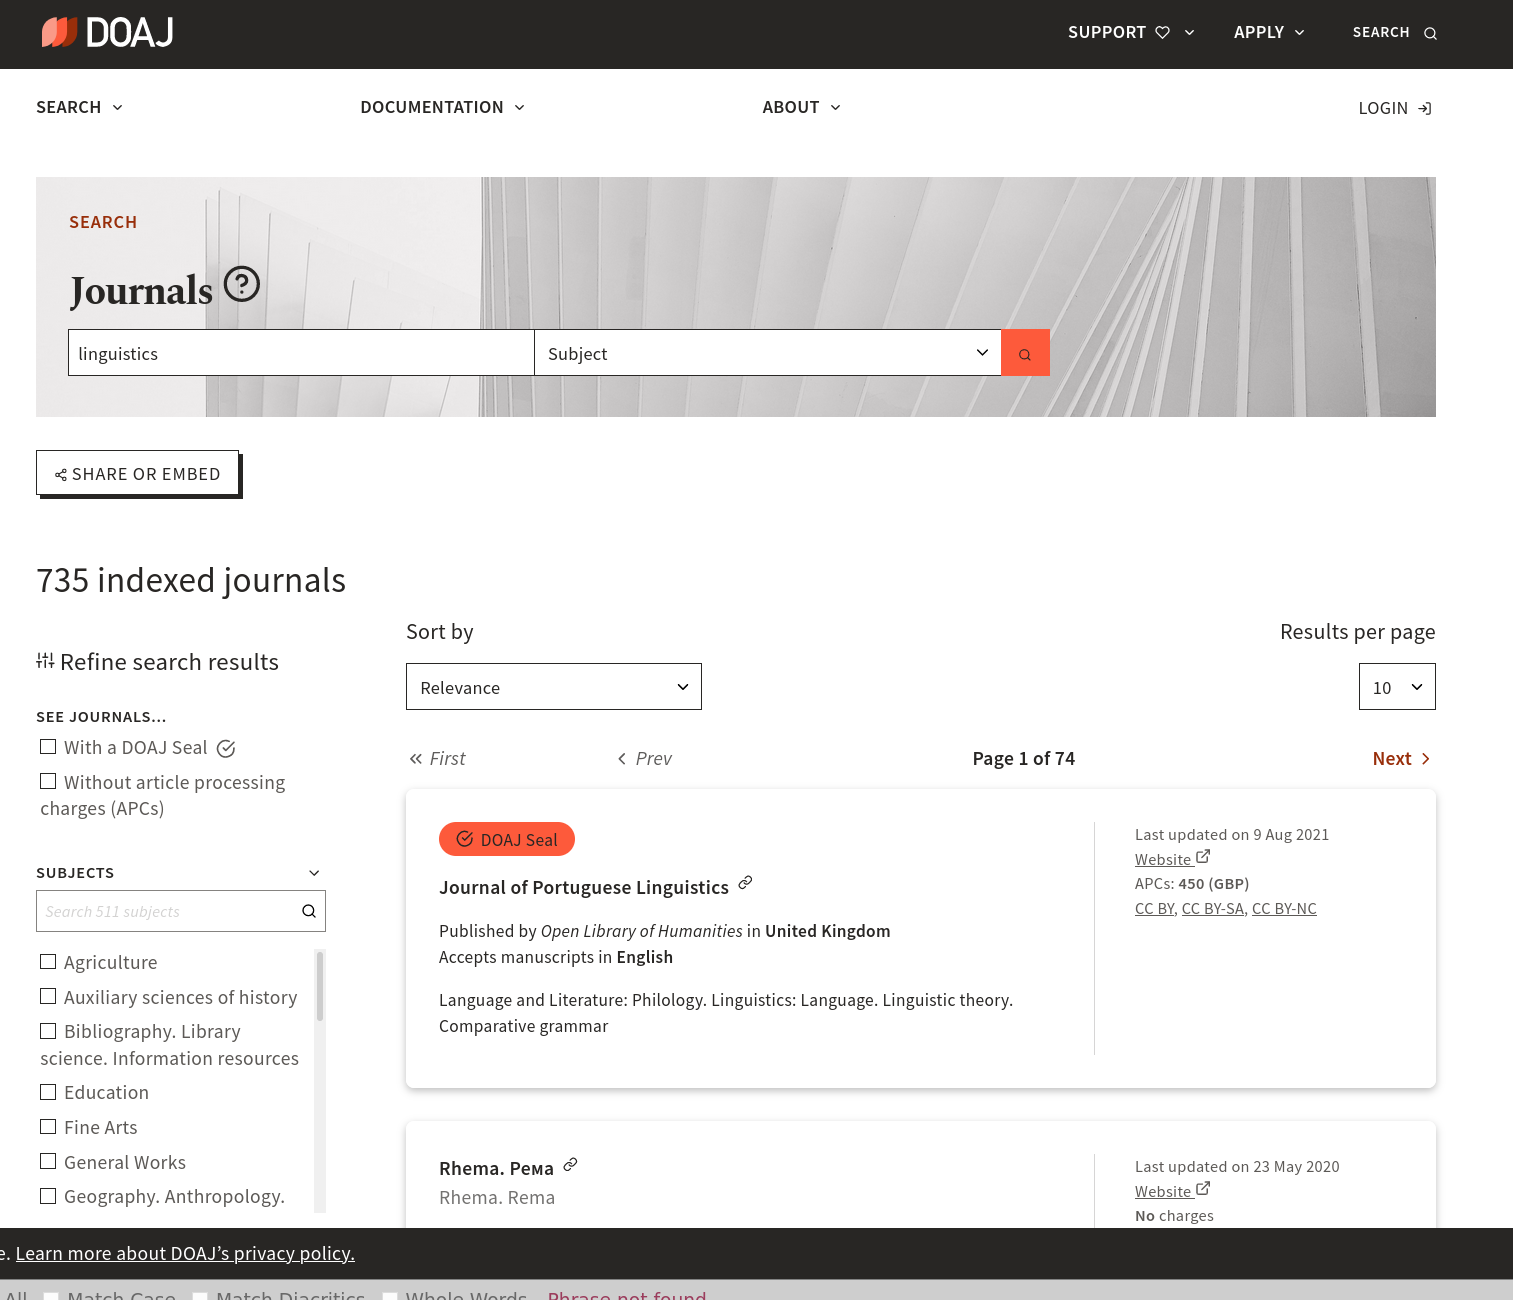
\includegraphics[height=1.2\textheight]{doaj.png}
}

\frame{
\frametitle{The Diamond Road\strut\\(also called Platinum)}
%   \includegraphics[height=.2\textheight]{./path/to/graphicsfile}
  \begin{itemize}
    \item Select a journal
    \item Get your paper accepted
    \item Pay \textbf{no} fee
    \item Readers don't have to pay anything to read the article
    \item A list of Diamond OA journals for linguistics can be found on oaling.wordpress.com
  \end{itemize}
}


% \frame{
% \frametitle{Think Check Submit}
%   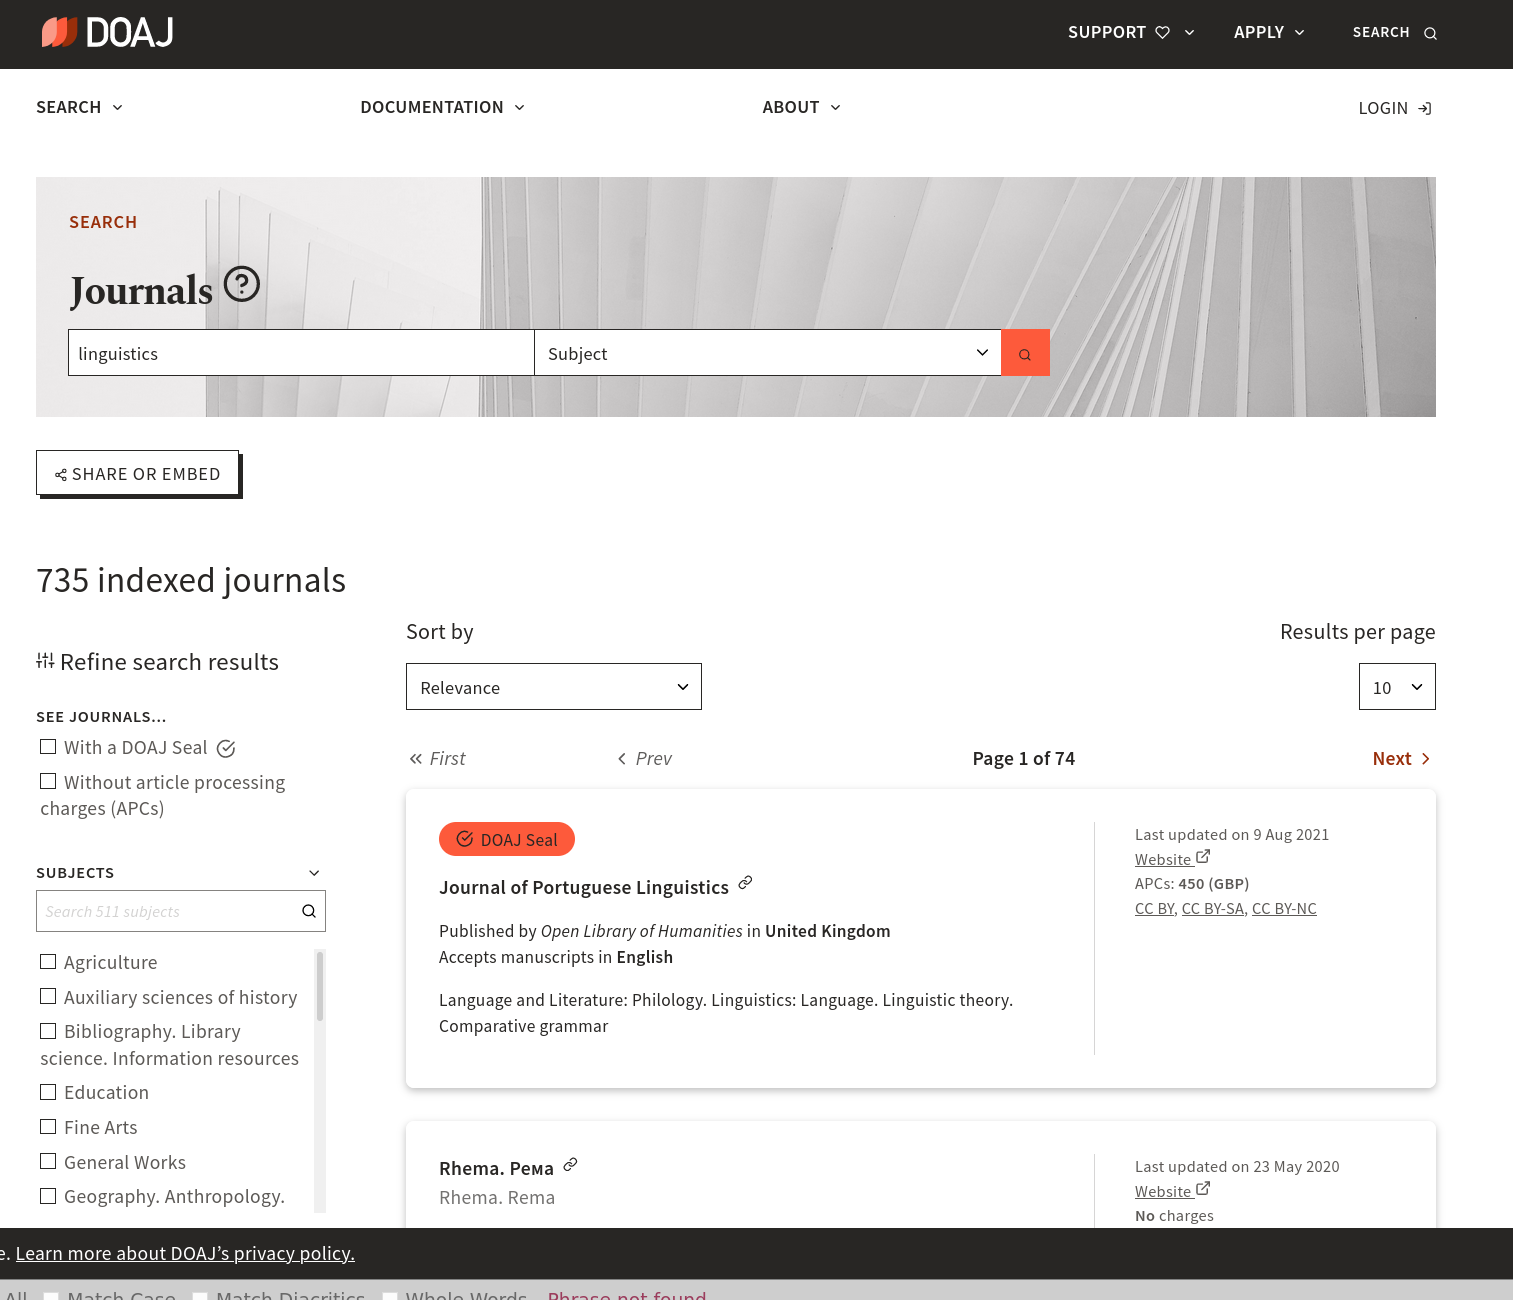
\includegraphics[height=\textheight]{doaj.png}
% }

\section{Books}
\frame{
\frametitle{Open Access books at\\ Language Science Press}
%   \includegraphics[height=.2\textheight]{./path/to/graphicsfile}
\begin{columns}
\column{7cm}
\begin{itemize}
    \item African Language Grammars and Dictionaries
    \begin{itemize}
      \item Dictionary + sketch grammar or grammar + word list.
      \item https://langsci-press.org/catalog/series/algad
    \end{itemize}
    \item Niger-Congo Comparative Studies
    \begin{itemize}
      \item https://langsci-press.org/catalog/series/nccs
    \end{itemize}
    \item Contemporary African Linguistics (from the Association for Contemporary African Linguistics)
    \begin{itemize}
      \item https://langsci-press.org/catalog/series/cal
    \end{itemize}
  \end{itemize}
\column{3cm}
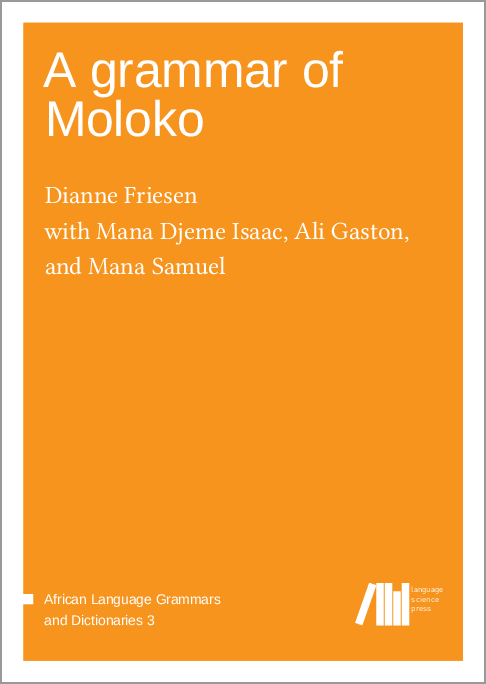
\includegraphics[height=2.2cm]{algad.png}\\
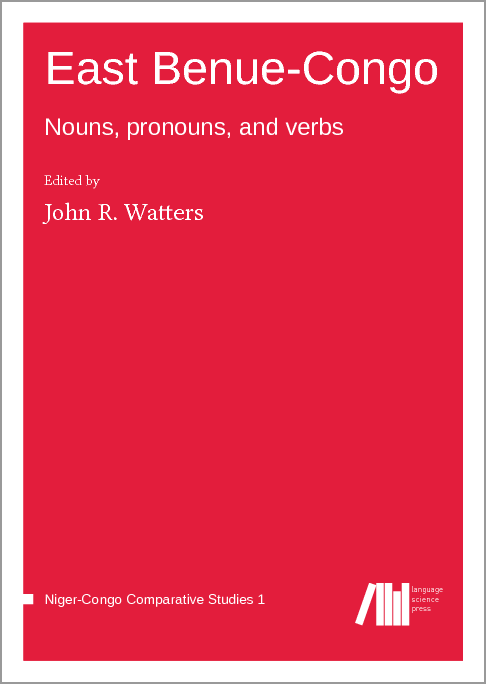
\includegraphics[height=2.2cm]{mcnc.png}\\
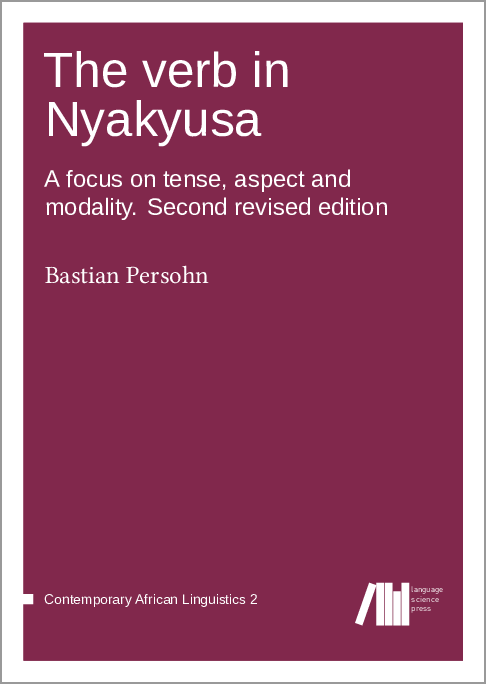
\includegraphics[height=2.2cm]{cal.png}
\end{columns}
}

\frame{
\frametitle{How to submit a book\strut\\ proposal}
%   \includegraphics[height=.2\textheight]{./path/to/graphicsfile}
  \begin{itemize}
    \item  identify relevant series and check their websites
    \begin{itemize}
      \item aims and scope
      \item requirements
      \item processes for proposals might be specified (or not)
    \end{itemize}
    \item contact series editor
    \item follow their instructions  (slightly different per series)
    \pause
    \item {\LARGE\color{red}\bfseries use a reference manager like Zotero when writing!}
  \end{itemize}
}

\frame{
\frametitle{Thank you!}
  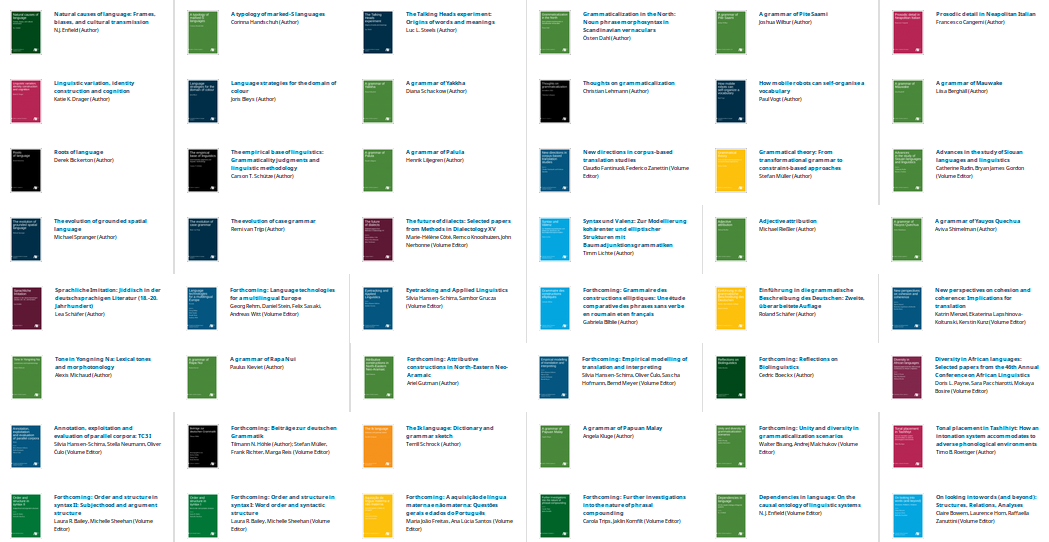
\includegraphics[height=\textheight]{catalog.png}
}

%\setcounter{framenumber}{\thelastpagemainpart}
\end{document}
